\kommentar{Reaktanzeintore (RET)}

\begin{karte}{Was ist ein Reaktanzeintor?}
	Ein Reaktanzeintor hat zwei Anschlüsse, besteht nur aus Reaktanzen und hat somit keine Wirkwiderstände.
	\\[10pt]
	\begin{minipage}{0.32\textwidth}
		Beispiel:
		\scalebox{.8}{%Autor: Simon Walker
%Version: 1.0
%Datum: 15.04.2020
%Lizenz: CC BY-NC-SA

\begin{circuitikz}
	%\HelpCords{-2}{2}{5}{-5}
	
	\draw
	%Knoten
	(2.3, 0) coordinate (n1)
	(2.3, -2) coordinate (n2)
	($(n1)+(0.7,0)$) coordinate (n11)
	($(n2)+(0.7,0)$) coordinate (n22)
	
	%Nur zu Hilfszwecken
%	(n1) node[above] {$n1$}
%	(n2) node[above] {$n2$}
%	(n11) node[above] {$n11$}
%	(n22) node[above] {$n22$}
	
	
	(0, 0) to [american inductor, o-] (n1)
	(n1) to[C, *-*] (n2)
	(n1) -- (n11) to[american inductor] (n22) -- (n2)
	(n2) to[short, -o] (0, -2)
	;
\end{circuitikz}}
	\end{minipage}
	\begin{minipage}{0.65\textwidth}
		Es wird zwischen minimalen und nicht minimalen Eintoren unterschieden. Nicht minimale Eintore können auf ein minimales Eintor reduziert werden ohne das die Änderung von aussen bemerkt wird.
	\end{minipage}\\[10pt]
	Da die RET nur aus $L$ und $C$ bestehen hat das RET bei $\omega = 0$ und bei $\omega \rightarrow \infty$ jeweils eine Pol oder eine Nullstelle.
\end{karte}

\begin{karte}{Wie sieht der Reaktanzverlauf des folgenden RET aus und was für ein Typ hat das RET?\\[5pt]
	%Autor: Simon Walker
%Version: 1.0
%Datum: 15.04.2020
%Lizenz: CC BY-NC-SA

\begin{circuitikz}
	%\HelpCords{-2}{2}{5}{-5}
	
	\draw
	%Knoten
	(2.3, 0) coordinate (n1)
	(2.3, -2) coordinate (n2)
	($(n1)+(0.7,0)$) coordinate (n11)
	($(n2)+(0.7,0)$) coordinate (n22)
	
	%Nur zu Hilfszwecken
%	(n1) node[above] {$n1$}
%	(n2) node[above] {$n2$}
%	(n11) node[above] {$n11$}
%	(n22) node[above] {$n22$}
	
	
	(0, 0) to [american inductor, o-] (n1)
	(n1) to[C, *-*] (n2)
	(n1) -- (n11) to[american inductor] (n22) -- (n2)
	(n2) to[short, -o] (0, -2)
	;
\end{circuitikz}}
	\begin{minipage}{0.55\textwidth}
		%Autor: Jürg Rast
%Datum: 04.04.2012
%Lizenz: CC BY-SA
%Grundversion von https://github.com/jrast/ELT4-Notizen/blob/master/tikzPictures/RET/ReaktanzLTyp.tex

%Geändert von: Simon Walker
%Datum: 15.04.2020
%Lizenz: CC BY-NC-SA


\usepgflibrary{shapes.misc}
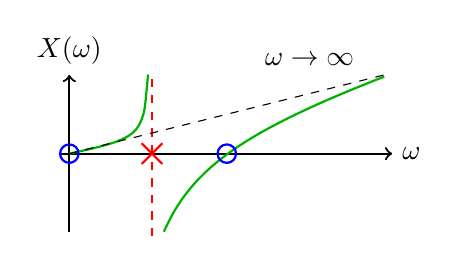
\begin{tikzpicture}[smooth, xscale=0.5, yscale=0.5]
% Achsen
\draw[->, thick] (-0.2,0) -- +(8.4,0) node[right] {$\omega$}; % Horizontal
\draw[->, thick] (0,-2) -- +(0,4) node[above] {$X(\omega)$}; % Vertikal

% Plots
\draw[color=green!70!black, thick] plot[domain=0:2] (\x,{\x/8+tan(\x*3/4 r)/8}); % Erster Tan
%\draw[color=green!70!black, thick] plot[domain=2.01:4.23] (\x,{tan(\x r)}); % zweiter Tan
\draw[color=green!70!black, thick] plot[domain=2.4:8] (\x,{ (\x/3.2) -3.8/(\x -1.01) }); % letzte kurve

% Poolstellen
\draw[dashed, thick, draw=red] (2.1,-2.1) -- +(0,4.2); % Poolstelle 1
\node[cross out, draw=red, thick] (wr1) at (2.1,0) {};


\draw[dashed] plot[domain=0:8] (\x, {\x/4});
\node (wL) at (6.1,2.4) {$\omega \rightarrow \infty$};

% Nullstellen
\node[rounded rectangle, draw=blue, thick] at(0,0) {};
\node[rounded rectangle, draw=blue, thick] at(4,0) {};
\end{tikzpicture}
	\end{minipage}
	\begin{minipage}{0.4\textwidth}
		Bei diesem Beispiel handelt sich um ein L-Typ
	\end{minipage}

	Als erstes wird das Verhalten des RET bei DC und bei sehr grossen Frequenzen analysiert. Für DC leiten beide Induktivitäten also ist dort eine NS. Für hohe Frequenzen sperrt die Erste Spule also ist dort eine PS.\\
	Da es bei dieser Schaltung um ein minimales RET handelt und aus drei Bauteilen besteht, hat der Reaktanzverlauf drei Pol/Null stellen. Diese treten abwechselnd auf.
\end{karte}

\begin{karte}{Wie sieht der Reaktanzverlauf des folgenden RET aus?\\[5pt]
		%Autor: Simon Walker
%Version: 1.0
%Datum: 15.04.2020
%Lizenz: CC BY-NC-SA

\begin{circuitikz}
	%\HelpCords{-2}{2}{5}{-5}
	
	\draw
	%Knoten
	(3, 0) coordinate (n1)
	(3, -2) coordinate (n2)
	($(n1)+(0.7,0)$) coordinate (n11)
	($(n2)+(0.7,0)$) coordinate (n22)
	(0.7, 0) coordinate (n3)
	(0.7, -2) coordinate (n4)
	(0, 0) coordinate (n5)
	(0, -2) coordinate (n6)
	
	
	%Nur zu Hilfszwecken
%	(n1) node[above] {$n1$}
%	(n2) node[above] {$n2$}
%	(n11) node[above] {$n11$}
%	(n22) node[above] {$n22$}
%	(n3) node[above] {$n3$}
%	(n4) node[above] {$n4$}
%	(n5) node[above] {$n5$}
%	(n6) node[above] {$n6$}
	
	(n5) to[short,o-] (n3)
	(n3) to[C, *-*] (n4)
	(n3) to [american inductor] (n1)
	(n1) to[C, *-*] (n2)
	(n1) -- (n11) to[american inductor] (n22) -- (n2)
	(n2) to[short, -o] (n6)
	;
\end{circuitikz}}
	\centering
	%Autor: Jürg Rast
%Datum: 04.04.2012
%Lizenz: CC BY-SA
%Grundversion von https://github.com/jrast/ELT4-Notizen/blob/master/tikzPictures/RET/ReaktanzPTyp.tex

%Geändert von: Simon Walker
%Datum: 15.04.2020
%Lizenz: CC BY-NC-SA

\usepgflibrary{shapes.misc}
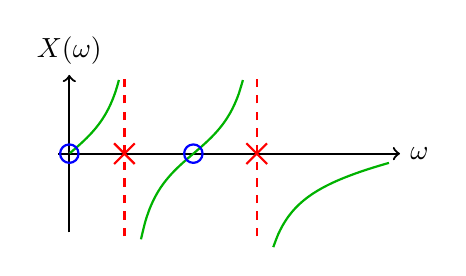
\begin{tikzpicture}[smooth, xscale=0.7, yscale=0.5]
% Achsen
\draw[->, thick] (-0.2,0) -- +(6.2,0) node[right] {$\omega$}; % Horizontal
\draw[->, thick] (0,-2) -- +(0,4) node[above] {$X(\omega)$}; % Vertikal

% Plots
\draw[color=green!70!black, thick] plot[domain=0.01:0.9] (\x, {tan( (\x *1.2) r )        }); % Erster Tan
\draw[color=green!70!black, thick] plot[domain=1.3:3.15] (\x,    {tan( (\x*1.2 -2.7) r)    }); % Erster Tan
\draw[color=green!70!black, thick] plot[domain=6.5:8.6] (\x-2.8,  { ((0.25 * \x) -1/(\x -6)) -2 }); % letzte kurve

% Poolstellen
\draw[dashed, thick, draw=red] (1,-2.1) -- +(0,4.2); % Poolstelle 1
\node[cross out, draw=red, thick] at (1,0) {};

\draw[dashed, thick, draw=red] (3.4,-2.1) -- +(0,4.2); % Poolstelle 2
\node[cross out, draw=red, thick] at (3.4,0) {};



% Nullstellen
\node[rounded rectangle, draw=blue, thick] at(0,0) {};
\node[rounded rectangle, draw=blue, thick] at(2.25,0) {};

\end{tikzpicture}\\
	\vspace{-5pt}
	\flushleft
	Als erstes wird das Verhalten des RET bei DC und bei sehr grossen Frequenzen analysiert. Für DC leiten beide Induktivitäten also ist dort eine NS. Für hohe Frequenzen leiten Beide Kapazitäten also ist dort ebenfalls NS.\\
	Da es bei dieser Schaltung um ein minimales RET handelt und aus vier Bauteilen besteht, hat der Reaktanzverlauf vier Pol/Null stellen. Diese treten abwechselnd auf.
\end{karte}

\begin{karte}{Ist folgendes RET ein minimales Eintor?\\[5pt]
		%Autor: Simon Walker
%Version: 1.0
%Datum: 15.04.2020
%Lizenz: CC BY-NC-SA

\begin{circuitikz}
	%\HelpCords{-2}{2}{5}{-5}
	
	\draw
	%Knoten
	(3, 0) coordinate (n1)
	(3, -2) coordinate (n2)
	($(n1)+(0.7,0)$) coordinate (n11)
	($(n2)+(0.7,0)$) coordinate (n22)
	(0.7, 0) coordinate (n3)
	(0.7, -2) coordinate (n4)
	(0, 0) coordinate (n5)
	(0, -2) coordinate (n6)
	
	
	%Nur zu Hilfszwecken
%	(n1) node[above] {$n1$}
%	(n2) node[above] {$n2$}
%	(n11) node[above] {$n11$}
%	(n22) node[above] {$n22$}
%	(n3) node[above] {$n3$}
%	(n4) node[above] {$n4$}
%	(n5) node[above] {$n5$}
%	(n6) node[above] {$n6$}
	
	(n5) to[short,o-] (n3)
	(n3) to[american inductor, *-*] (n4)
	(n3) to [american inductor] (n1)
	(n1) to[C, *-*] (n2)
	(n1) -- (n11) to[american inductor] (n22) -- (n2)
	(n2) to[short, -o] (n6)
	;
\end{circuitikz}}
	Nein! Denn es hat ein Ring aus Induktivitäten. In diesem Ring kann ein Strom fliesen. Dieser Strom ist von aussen nicht sichtbar. Eine Induktivität kann ersatzlos gestrichen werden, wenn dementsprechend die anderen Induktivitäten angepasst werden. Danach ist von aussen kein Unterschied feststellbar.\\
	\begin{center}
		%Autor: Simon Walker
%Version: 1.0
%Datum: 15.04.2020
%Lizenz: CC BY-NC-SA

\begin{circuitikz}
	%\HelpCords{-2}{2}{5}{-5}
	
	\draw
	%Knoten
	(3, 0) coordinate (n1)
	(3, -2) coordinate (n2)
	($(n1)+(0.7,0)$) coordinate (n11)
	($(n2)+(0.7,0)$) coordinate (n22)
	(0.7, 0) coordinate (n3)
	(0.7, -2) coordinate (n4)
	(0, 0) coordinate (n5)
	(0, -2) coordinate (n6)
	

	
	%Nur zu Hilfszwecken
%	(n1) node[above] {$n1$}
%	(n2) node[above] {$n2$}
%	(n11) node[above] {$n11$}
%	(n22) node[above] {$n22$}
%	(n3) node[above] {$n3$}
%	(n4) node[above] {$n4$}
%	(n5) node[above] {$n5$}
%	(n6) node[above] {$n6$}
	
	(n5) to[short,o-] (n3)
	(n3) to[american inductor, *-*] (n4)
	(n3) to [american inductor] (n1)
	(n1) to[C, *-*] (n2)
	(n1) -- (n11) to[american inductor] (n22) -- (n2)
	(n2) to[short, -o] (n6)
	;
	
	\draw[very thick, blue, rounded corners=5mm]
	(n3) -- (n11) -- (n22) -- (n4) -- cycle;
\end{circuitikz}
	\end{center}
\end{karte}

\begin{karte}{Welche Eigenschaften eines RET sind in der Praxis am unwahrscheinlichsten?}
	Es gibt zwei Probleme:
	\begin{compactitem}
		\item Impedanz wird nie 0 erreichen
		\item Die Impedanz kann nicht undendlich gross werden.
	\end{compactitem}
	Allerdings wird die Impedanz sich nicht komplett anders verhalten als die Reaktanz.
	%Autor: Simon Walker
%Version: 1.0
%Datum: 18.04.2020
%Lizenz: CC BY-NC-SA

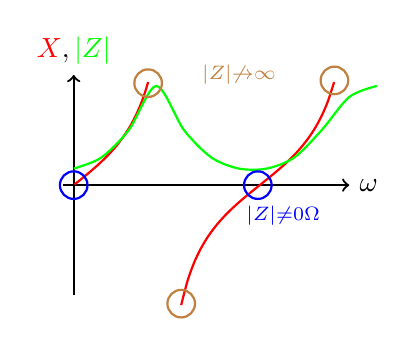
\begin{tikzpicture}[smooth, xscale=0.7, yscale=0.7]
% Achsen
\draw[->, thick] (-0.2,0) -- +(5.2,0) node[right] {$\omega$}; % Horizontal
\draw[->, thick] (0,-2) -- +(0,4) node[above] {$\color{red}X \color{black}, \color{green} \left|Z\right|$}; % Vertikal

% Plots
\draw[color=red, thick] plot[domain=0.01:0.9] (\x*1.5,{tan((\x *1.2) r )}); % Erster Tan
\draw[color=red, thick] plot[domain=1.3:3.15] (\x*1.5,{tan((\x*1.2 -2.7) r)}); % Zweiter Tan
%Impedanz
%\draw[color=green, thick] plot[domain=0.01:0.9] (\x*1.5,{0.3+0.6*tan((\x *1.2) r )}); % Erster Tan

\draw [green, thick] plot [smooth] coordinates{
(0, 0.3) (0.5, 0.5) (1, 1) 
(1.5, 1.8)  (2, 1) (2.5, 0.5)
(3, 0.3) (3.5, 0.3) (4, 0.5) 
(4.5, 1) (5, 1.6) (5.5, 1.8)};


\draw [blue, thick] (3.34, 0) circle[radius=0.25];
\draw [blue, thick] (0, 0) circle[radius=0.25];
\draw [brown, thick] (1.35, 1.85) circle[radius=0.25];
\draw [brown, thick] (1.95, -2.15) circle[radius=0.25];
\draw [brown, thick] (4.73, 1.9) circle[radius=0.25];

\node [below] at (3.8, -0.2) {$\scriptstyle \color{blue} \left|Z\right| \ne 0 \Omega$};
\node at (3, 2) {$\scriptstyle \color{brown} \left|Z\right| \not\rightarrow \infty$};

\end{tikzpicture}

\end{karte}


